\mysection{目的}
\begin{enumerate}
  \setlength{\parskip}{0cm} % 段落間
  \setlength{\itemsep}{0cm} % 項目間
  \item オシロスコープの使い方を確認するとともに、ディジタルオシロスコープの使い方を確認する。
  \item ディジタルオシロスコープで保存した波形データを使用してフーリエ級数展開を行うことで、数値積分のやり方や表計算ソフトウェアの使い方を学ぶとともに、フーリエ級数展開について理解する。
\end{enumerate}

\mysection{原理}
ディジタルオシロスコープとは、波形観測に用いられる計測器具である。その構成を図\ref{im1}に示す。(矢印は入力信号の向きを示す。)

\begin{figure}[htbp]
  \begin{center}
  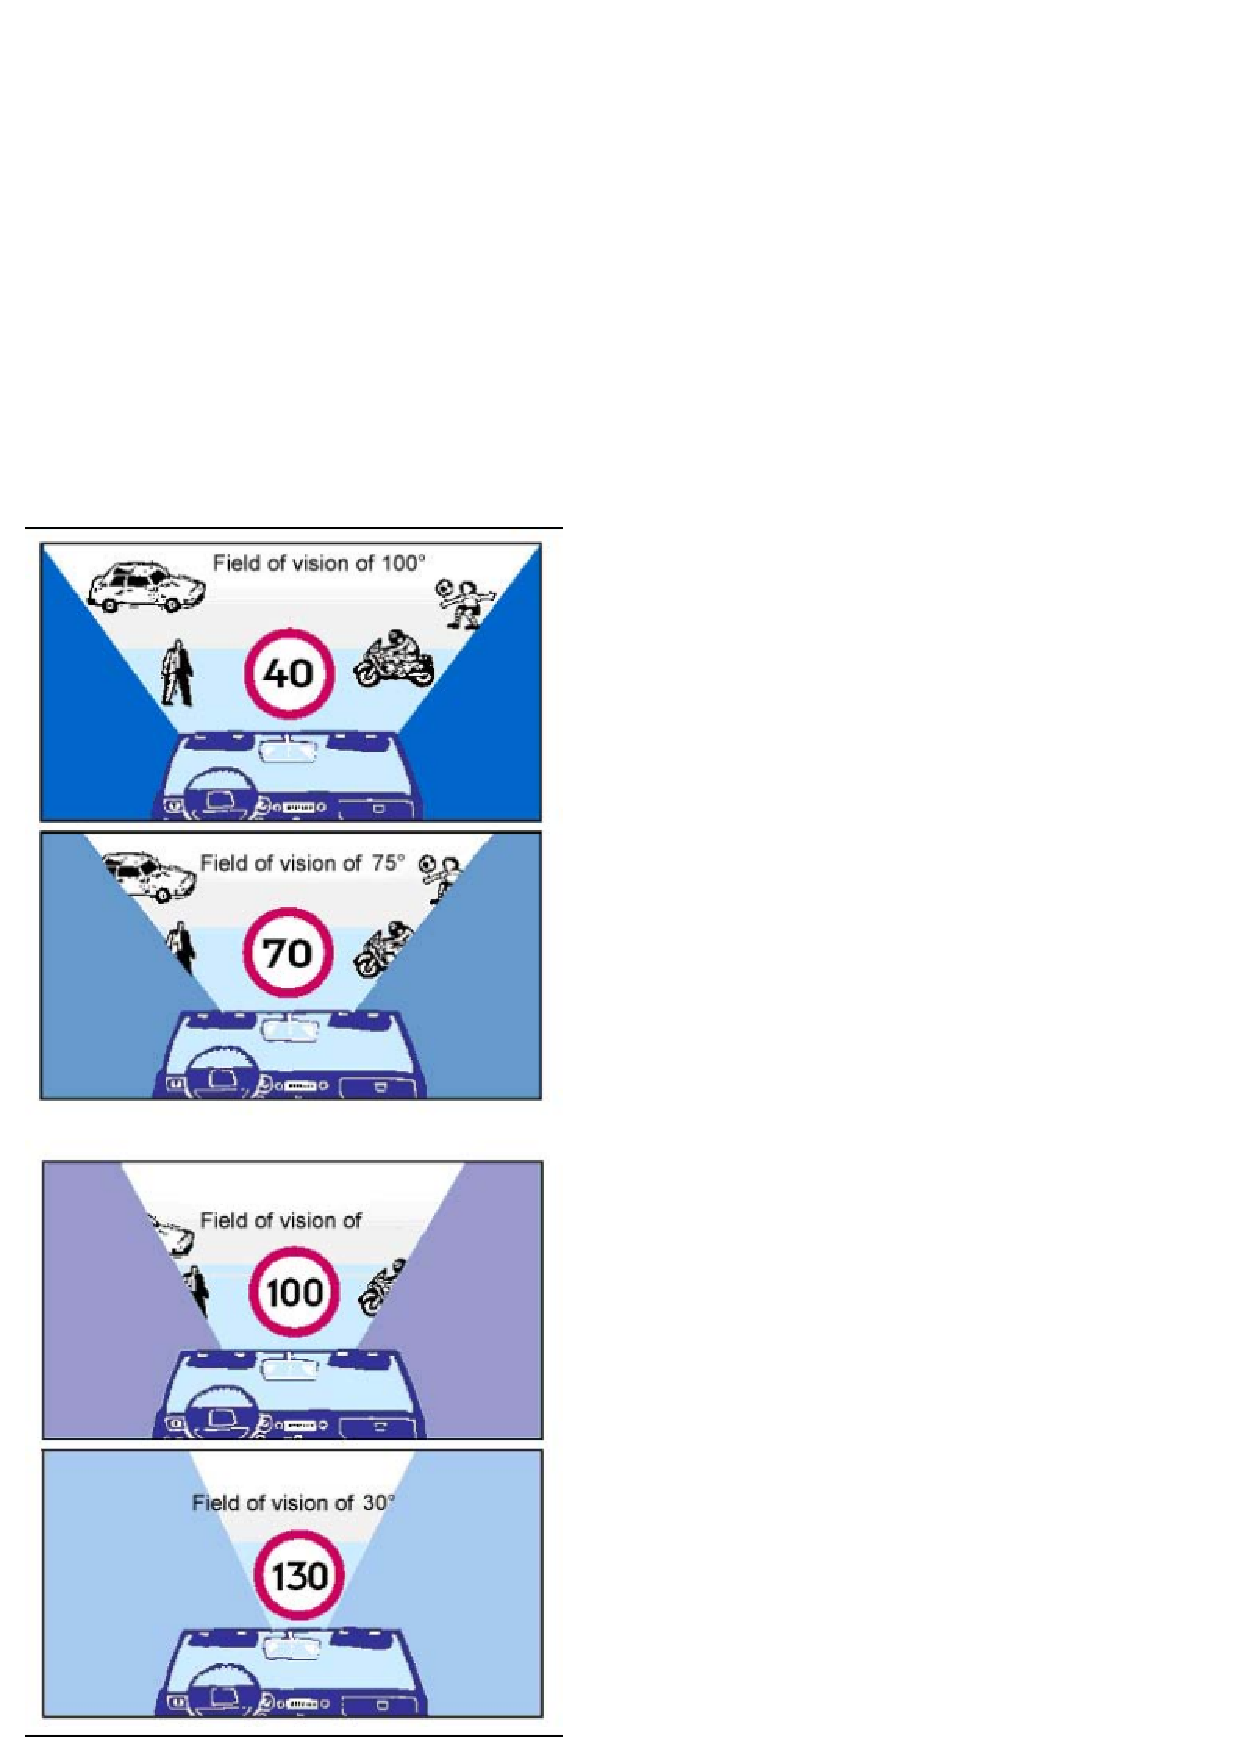
\includegraphics[width=.5\linewidth]{img/1.jpg}
  \caption{ディジタルオシロスコープの基本構成}
  \label{im1}
  \end{center}
\end{figure}

\mysubsection{ディジタルオシロスコープの動作原理について}
ディジタルオシロスコープは、観測信号(アナログ信号)をA/D変換によってディジタル信号に変換し、
そのデータをメモリに保存してから波形を表示する。ディジタル信号で画面に線を描画するためには、観測信号と掃引信号を同期する必要がある。
同期の取り方は、トリガ同期方式を用いる。トリガ同期方式は、測定したい波形の振幅よりも少し小さい振幅にトリガレベルを設定することによって、
入力信号の振幅がトリガレベルを超えたときに掃引信号が発生する方式である。
また、ディジタルオシロスコープにおいて、トリガレベルは自由に設定できる。

\mysubsection{AD変換器について}
アナログ信号をディジタル信号に変換することをA/D変換という。 
A/D変において、\textbf{\textgt{サンプリング (標本化)・量子化・符号化}} の操作を行う必要がある。
サンプリング (標本化)・量子化を図\ref{im2}に示す。

\begin{figure}[htb]
  \begin{center}
  \subfigure[サンプリング(標本化)]{
  \includegraphics[width=.45\columnwidth]{img/2.jpg}
  }
  \subfigure[量子化]{
  \includegraphics[width=.45\columnwidth]{img/3.jpg}
  }
  \caption{サンプリング・量子化について}
  \label{im2}
  \end{center}
\end{figure}

\begin{description}
  \setlength{\parskip}{0cm} % 段落間
  \setlength{\itemsep}{0cm} % 項目間
  \item[サンプリング] 時間的に連続な波形から時間間隔$\varDelta t$ごとに波形の振幅を取り出す操作のことである。
  $\varDelta t$を\textbf{\textgt{サンプリング間隔}}、その逆数を\textbf{\textgt{サンプリング周波数}}という。
  サンプリング定理によるとサンプリング周波数を元のアナログ信号に含まれている最大周波数の2倍以上にすれば、元の波形を再現することができる。
  \item[量子化] サンプリングした波形の振幅を分割して、最も近い整数を割り当てる操作のことである。
  量子化前後の誤差を\textbf{\textgt{量子化誤差}}といい、量子化に波形の分割数が少ないと、量子化誤差が大きくなる。
  \item[符号化] 量子化された整数(10進数)を2進数に変換する操作である。
\end{description}

\mysubsection{本実験で使用した表計算ソフトについて}
表計算を行う際、実際にデータを入力する一桝をセルという。
各セルに計算式を表す \verb|“=”|(イコール)の記号を先頭に入力し、
算術計算の式を入力することによってそのセルに、その演算結果を入力できる。

\mysubsection{フーリエ級数展開について}
周期関数$f(t)$ (周期$T$)を、
次の式のように三角関数の項と$b_0$の式で表すことができることを示す。
\begin{screen}
  \begin{equation}
    f(t) = b_0+\sum_{n = 1}^{\infty} b_n \cos n\omega t + \sum_{n = 1}^{\infty} a_n \sin n\omega t \label{eq1}
  \end{equation}
\end{screen}
  
式\eqref{eq1}の、$b_0$、$a_n$、$b_n$をフーリエ係数という。また、フーリエ係数は、それぞれ、式\eqref{eq2}~\eqref{eq4}のように表すことができる。

\begin{screen}  
  \begin{gather}
    b_0 = \frac{1}{T}\int_{0}^{T}f(t) \,dt \label{eq2} \\
    b_n = \frac{1}{T}\int_{0}^{T}f(t)\cos n\omega t \,dt \label{eq3} \\
    a_n = \frac{1}{T}\int_{0}^{T}f(t)\sin n\omega t \,dt \label{eq4}
  \end{gather}
\end{screen}

\mysubsection{数値積分について}
時間間隔が$\varDelta t$で標本化された関数$f_i = f(t_i) (i = 1, 2, 3, \dots N)$の定積分は、式\eqref{eq5}で近似できる。
数値積分で近似している部分を図\ref{im3}に長方形で示す。
\begin{screen} 
  \begin{equation}
    \int_{t_1}^{t_n}f(t) \,dt = \int_{t_n}^{t_{N-1}}f(t) \,dt + \varDelta t \sum_{i = 1}^{N-1}f_i \label{eq5}
  \end{equation}
\end{screen}

\begin{figure}[htbp]
  \begin{center}
  \includegraphics[width=.5\linewidth]{img/4.jpg}
  \caption{数値積分}
  \label{im3}
  \end{center}
\end{figure}